% =====================================================================
% Design Review — RSA32 APB
% Compilar: pdflatex design_review.tex (duas vezes)
% =====================================================================
\documentclass[aspectratio=169,10pt,t]{beamer}

\usepackage[utf8]{inputenc}
\usepackage[T1]{fontenc}
\usepackage[brazilian]{babel}
\usepackage{lmodern}
\usepackage[scaled=0.95]{helvet}
\renewcommand{\familydefault}{\sfdefault}
\usepackage{tabularx}
\usepackage{array}

\newcommand{\tmLogoPath}{..}   % logos ficam em docs/
\usetheme{TcheMOS}

% Repositório: evidências na branch FEAT-UVM
\newcommand{\tmRepo}{https://github.com/TCHE-MOS/RSA32_APB/tree/FEAT-UVM/docs/entregaveis}

\title[Design Review · RSA\_APB]{Design Review — RSA\_APB}
\subtitle{Coprocessador RSA · AMBA~3 APB · TSMC 28\,nm}
\author[Matheus Grossi · Milena Resmer]{Matheus Grossi \quad·\quad Milena Resmer}
\manager{Alcides Costa}
\institute{TchêMOS — Semiconductor Design House}
\date{Novembro de 2026}

\begin{document}

% ---------------------------------------------------------------------
\begin{frame}[plain,noframenumbering]
  \titlepage
\end{frame}

% =====================================================================
% Entregáveis
% =====================================================================
\begin{frame}{Entregáveis do projeto}{Critérios de aceitação}
  \scriptsize
  \renewcommand{\arraystretch}{1.18}
  \begin{tabularx}{\textwidth}{@{}>{\bfseries\color{tmCafe}}l X >{\raggedright\arraybackslash}p{0.36\textwidth}@{}}
    \toprule
    \textbf{ID} & \textbf{Entregável} & \textbf{Requisito de aceitação} \\
    \midrule
    E01 & Coprocessador RSA de 32 bits e respectivo testbench em SystemVerilog & Código-fonte disponível e funcional \\
    E02 & Relatório de equivalência lógica entre as implementações RSA de 4 bits em Verilog e SystemVerilog & Equivalência lógica comprovada \\
    E03 & Relatório de simulação funcional do \texttt{rsa\_core32b} & Testes executados com sucesso \\
    E04 & Ambiente de verificação UVM para a interface \texttt{rsa\_apb} & Ambiente funcional e executável \\
    E05 & Relatório de simulação funcional da interface RSA\_APB de 32 bits & Testes funcionais aprovados \\
    E06 & Relatório de cobertura funcional da interface RSA\_APB de 32 bits & Métricas apresentadas e correlacionadas ao plano de verificação \\
    E07 & Gate-level netlist mapeado para a tecnologia TSMC de 28\,nm & Netlist gerado corretamente pelo Cadence Genus \\
    E08 & Relatório de análise estática de temporização (STA) & Ausência de violações de setup nos caminhos analisados (TNS = WNS = 0) \\
    E09 & Relatório de simulação pós-síntese da interface RSA\_APB, com anotação de atrasos SDF & Testes aprovados, sem violações de temporização reportadas durante a simulação \\
    E10 & Scripts de automação do fluxo de desenvolvimento & Execução reproduzível das etapas e geração dos respectivos artefatos \\
    \bottomrule
  \end{tabularx}
\end{frame}

% =====================================================================
% Rascunho da arquitetura
% Fonte: docs/rascunho_da_arquitetura.png
% =====================================================================
\begin{frame}{Rascunho da arquitetura}{Concepção inicial do periférico RSA\_APB}
  \vspace*{-0.45cm}
  \centering
  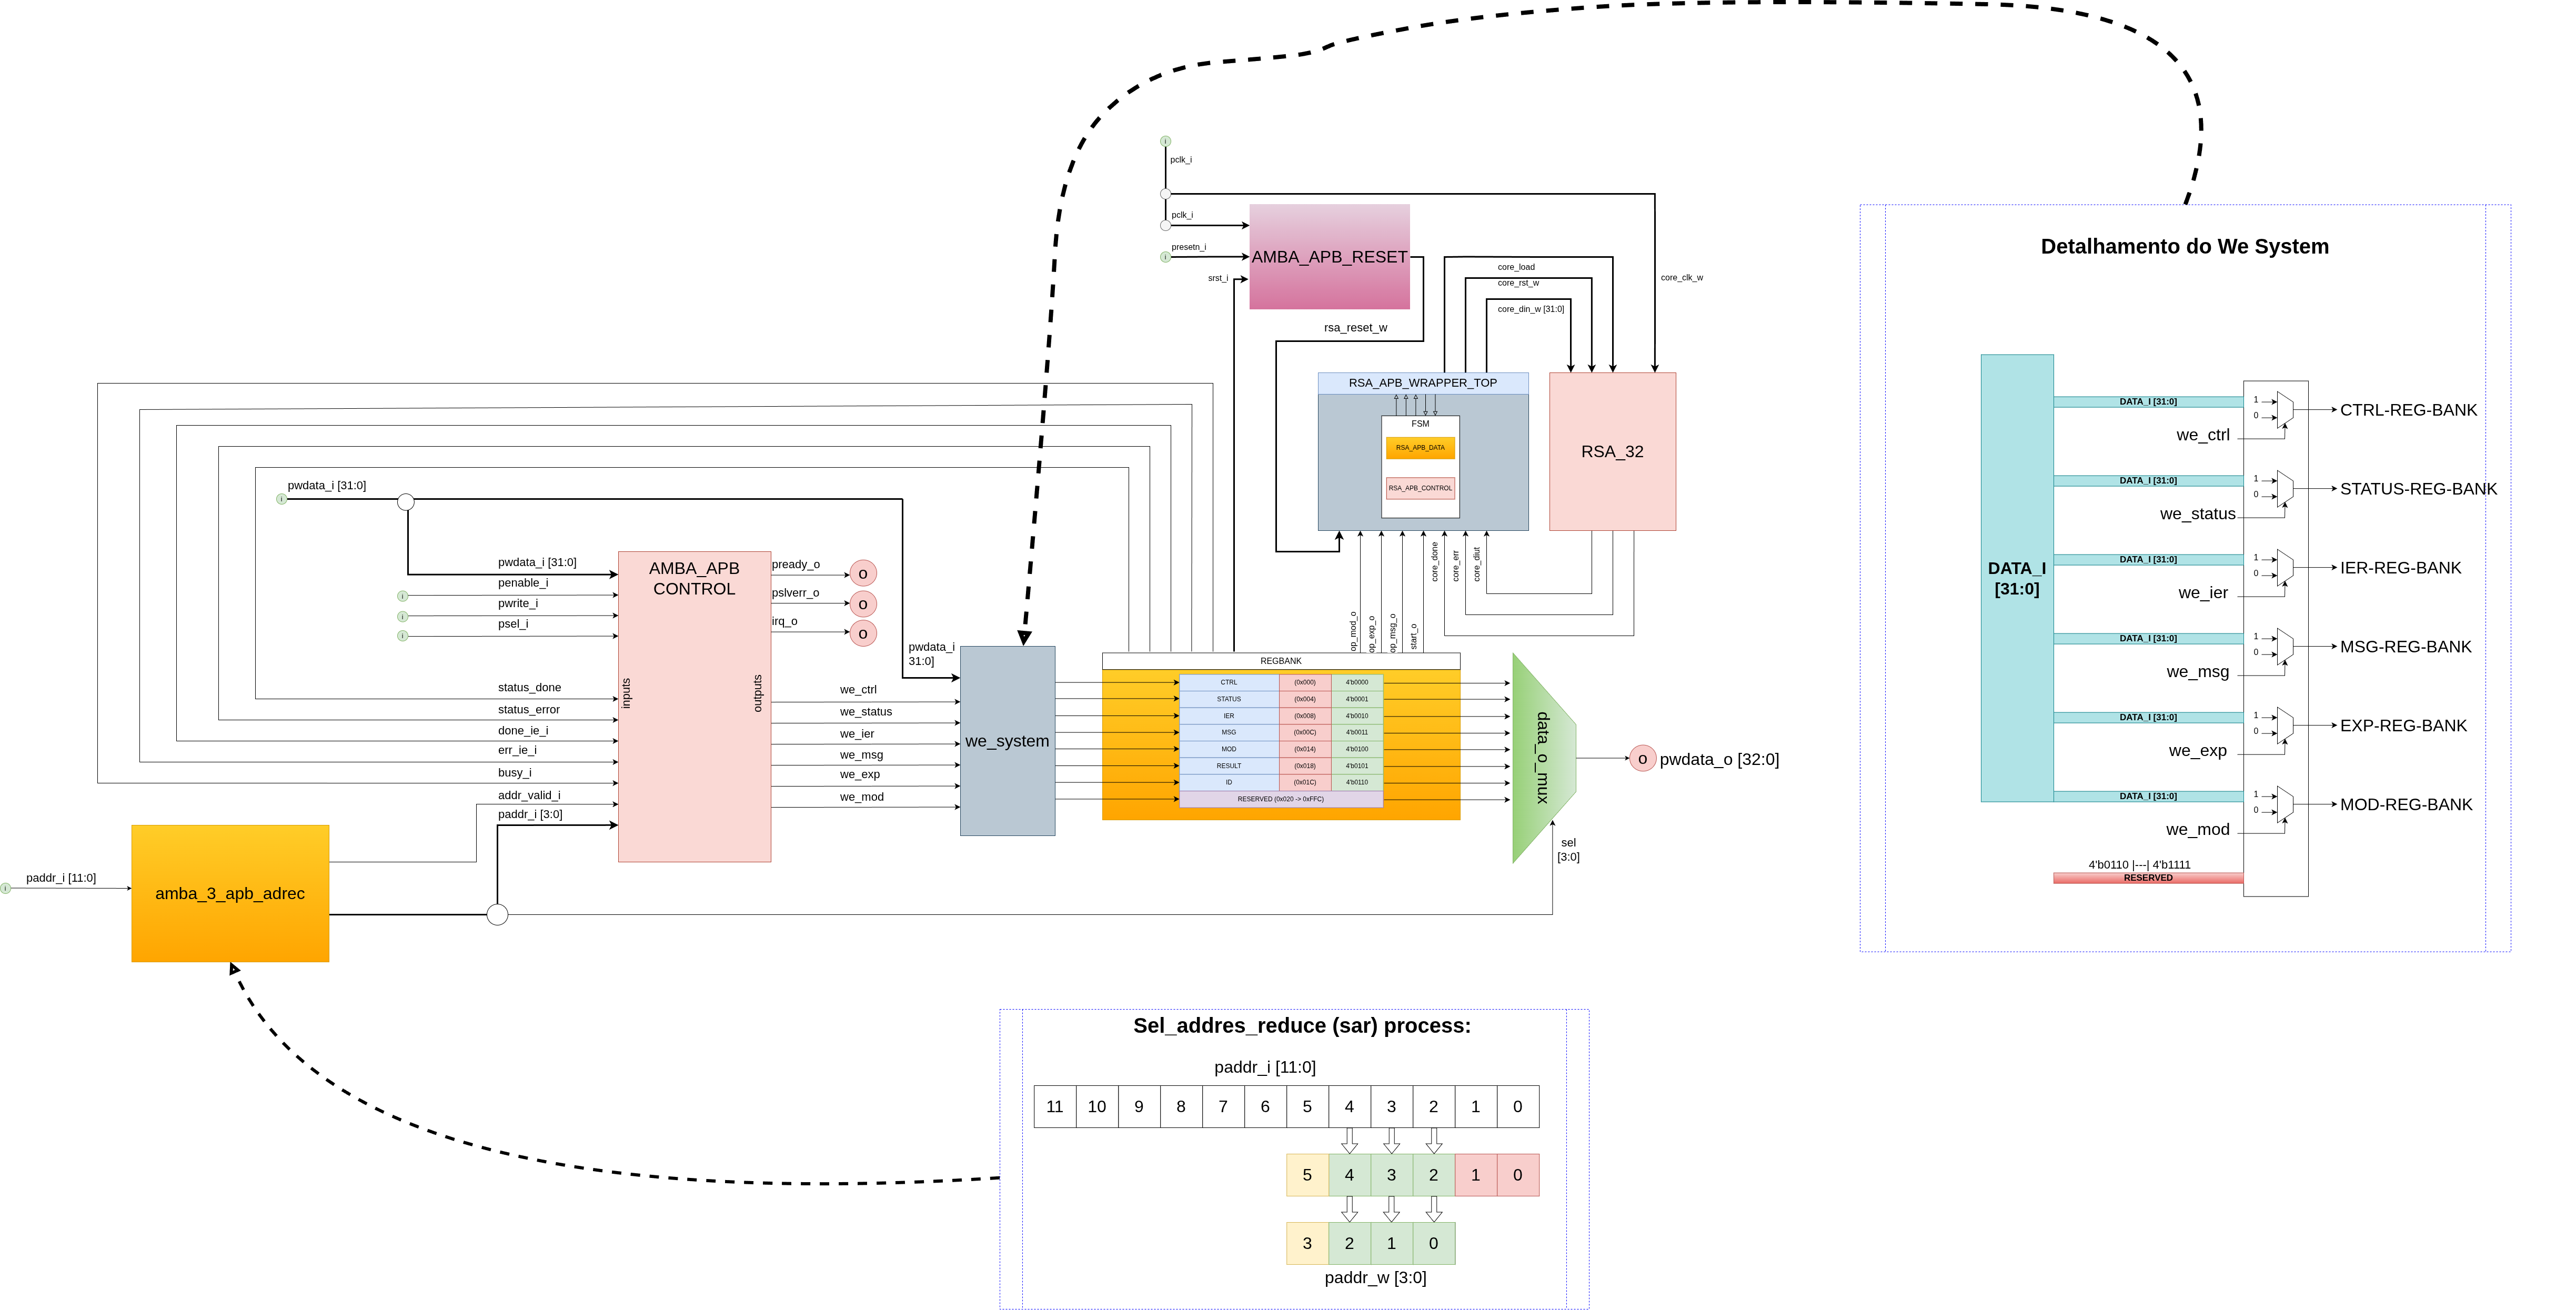
\includegraphics[width=\textwidth,height=6.7cm,keepaspectratio]{figuras/rascunho_da_arquitetura.png}
\end{frame}

% =====================================================================
% Diagrama de blocos do topo
% Fonte: schematic_generator/esquematico/saida/esquematicos_apb_rsa.pdf (pág. 2)
% =====================================================================
\begin{frame}{Diagrama de blocos do topo}{\texttt{amba\_3\_apb\_rsa\_apb\_top} — esquemático RTL elaborado}
  \vspace{0.1cm}
  \centering
  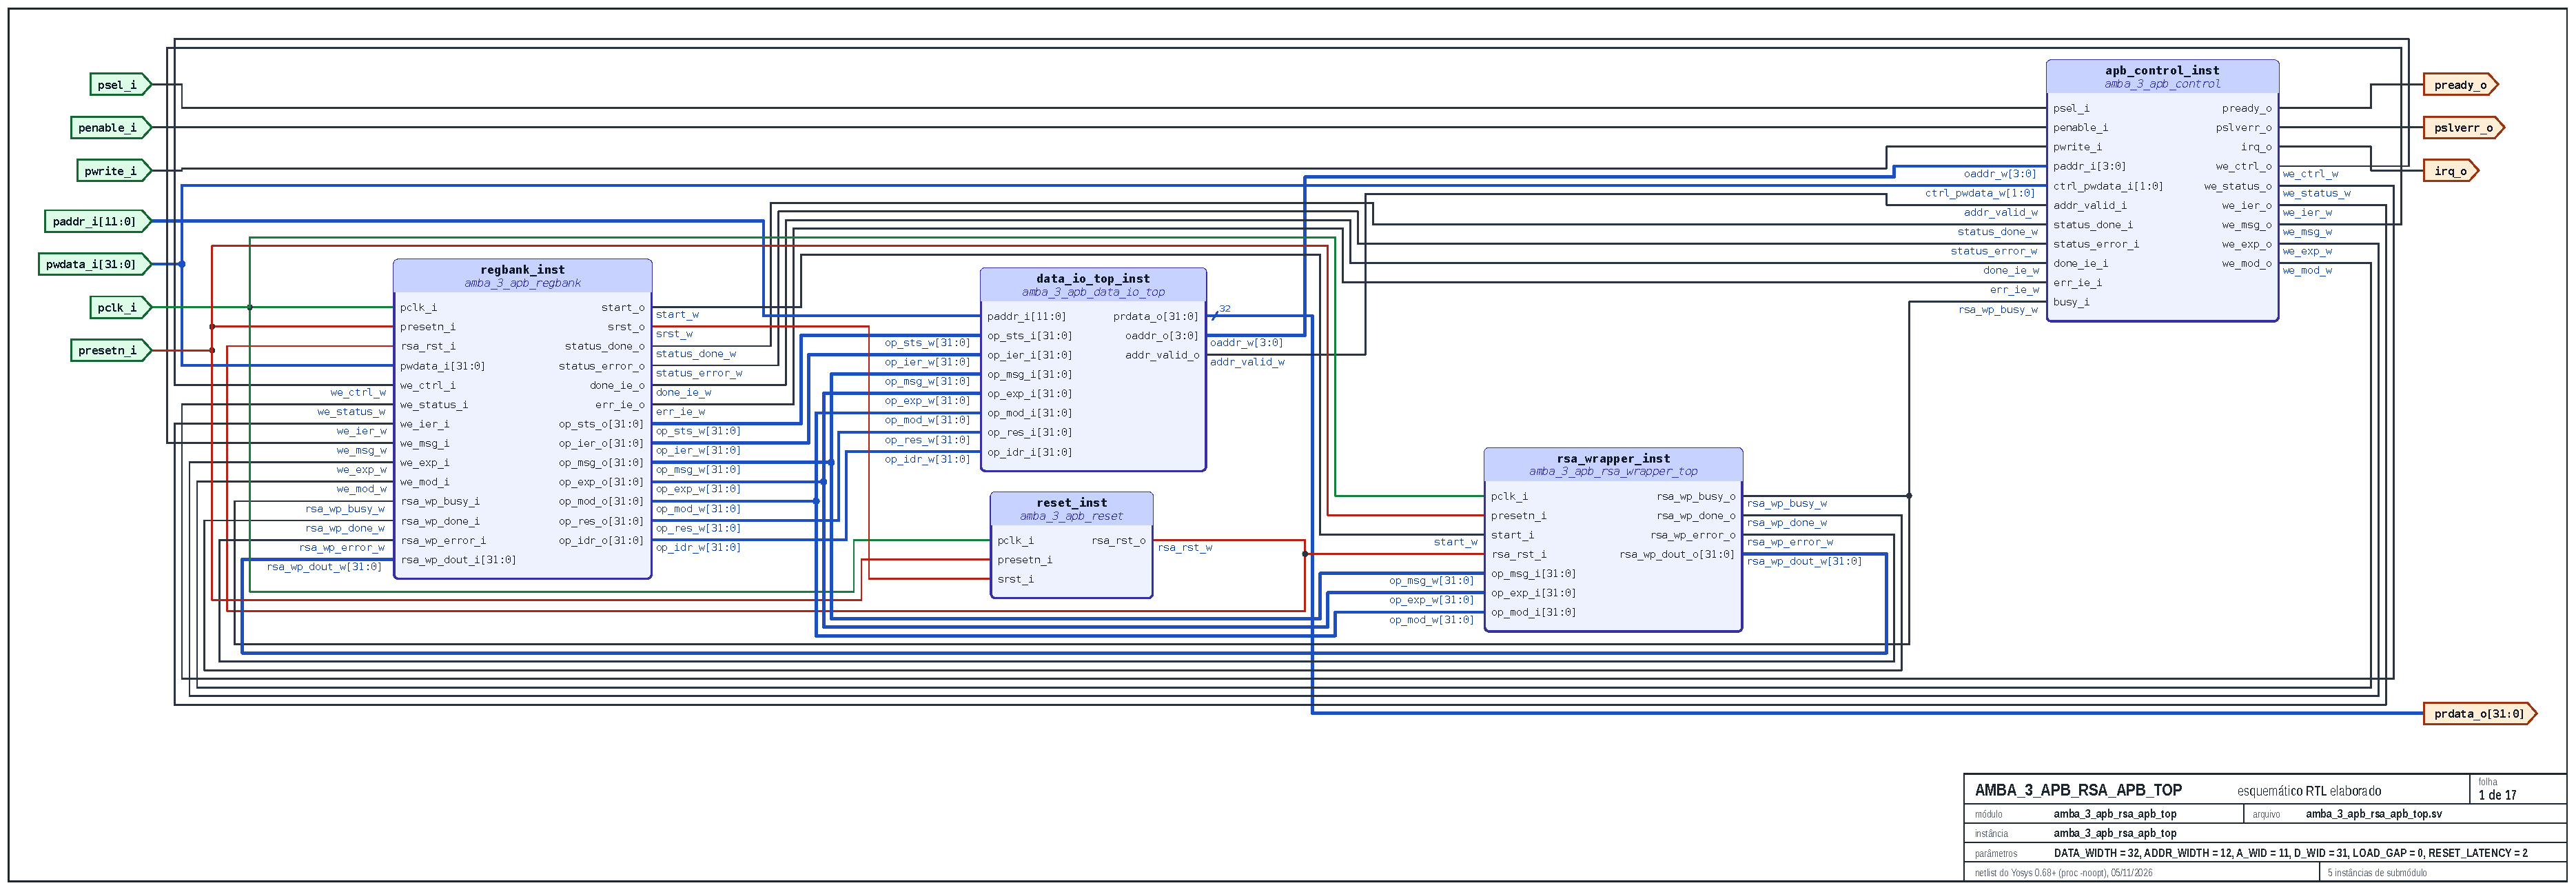
\includegraphics[width=\textwidth]{figuras/diagrama_topo.pdf}
\end{frame}

% ---------------------------------------------------------------------
% E01
% ---------------------------------------------------------------------
\begin{frame}{E01~— Coprocessador RSA de 32 bits e testbench}
  \begin{block}{Entregável}
    Coprocessador RSA de 32 bits e respectivo testbench em SystemVerilog
  \end{block}
  \begin{exampleblock}{Requisito de aceitação}
    Código-fonte disponível e funcional
  \end{exampleblock}
  \vspace{0.1cm}
  {\color{tmDourado}\rule{\linewidth}{0.5pt}}\\[0.05cm]
  {\small\color{tmVermelho}\textbf{Pergunta da revisão:}} {\small\itshape O módulo \texttt{rsa\_core32b} possui um testbench funcional?}
  % TODO: evidências e status
\end{frame}

% ---------------------------------------------------------------------
% E02
% ---------------------------------------------------------------------
\begin{frame}{E02~— Equivalência lógica RSA 4 bits}{Cadence Conformal LEC · golden Verilog $\times$ revised SystemVerilog}
  \begin{columns}[T]
    \begin{column}{0.5\textwidth}
      \begin{block}{Entregável}
        \small Relatório de equivalência lógica entre as implementações RSA de 4 bits em Verilog e SystemVerilog
      \end{block}
      \begin{exampleblock}{Requisito de aceitação \hfill \tmOK}
        \small Equivalência lógica comprovada
      \end{exampleblock}
      {\color{tmDourado}\rule{\linewidth}{0.5pt}}\\[0.05cm]
      {\scriptsize\color{tmVermelho}\textbf{Pergunta da revisão:}} {\scriptsize\itshape O RSA de 4 bits do cliente (Verilog) é logicamente equivalente à versão em SystemVerilog? Apresente as evidências.}
    \end{column}
    \begin{column}{0.46\textwidth}
      \tmVeredito{tmOliva}{EQUIVALÊNCIA COMPROVADA — PASS}{94 de 94 pontos equivalentes · 0 não equivalentes · 0 abortados}
      \vspace{0.15cm}
      \scriptsize
      \begin{tabular}{@{}ll@{}}
        \toprule
        Golden   & \texttt{src/vlog/rsa\_core.v} (\texttt{-verilog2k}) \\
        Revised  & \texttt{src/sv/rsa\_core.sv} (\texttt{-systemverilog}) \\
        Topo     & \texttt{rsa\_core} \\
        Ferramenta & Conformal 23.20-s200 \\
        Modo     & \texttt{lec}, \texttt{compare\_effort high} \\
        Pontos   & \texttt{add\_compared\_points -all} \\
        Saída    & \texttt{Compare Results: PASS} (código 0) \\
        \bottomrule
      \end{tabular}
    \end{column}
  \end{columns}
  \tmRepoLink{\tmRepo/E02}{Evidências E02 no GitHub}
\end{frame}

\begin{frame}{E02~— Equivalência lógica RSA 4 bits}{Mapeamento, comparação e ressalvas}
  \begin{columns}[T]
    \begin{column}{0.48\textwidth}
      \scriptsize
      \textbf{\color{tmCafe}Estrutura elaborada (idêntica nas duas versões)}\\[0.1cm]
      \begin{tabular}{@{}lrr@{}}
        \toprule
        Métrica & Golden & Revised \\
        \midrule
        Módulos de projeto & 5 & 5 \\
        Entradas / saídas primárias & 7 / 7 & 7 / 7 \\
        Primitivas (nível de bit) & 866 & 866 \\
        Flip-flops & 88 & 88 \\
        \bottomrule
      \end{tabular}\\[0.25cm]
      \textbf{\color{tmCafe}Comparação formal}\\[0.1cm]
      \begin{tabular}{@{}lrrr@{}}
        \toprule
        Pontos & PO & DFF & Total \\
        \midrule
        Equivalentes & 7 & 87 & \textbf{94} \\
        Não equivalentes & 0 & 0 & 0 \\
        Abortados & 0 & 0 & 0 \\
        \bottomrule
      \end{tabular}
    \end{column}
    \begin{column}{0.48\textwidth}
      \begin{itemize}\small
        \item 88 DFFs por versão: 87 mapeados e provados; \textbf{1 inalcançável} (\emph{unreachable}) em ambas — não é ponto não equivalente.
        \item \texttt{report\_verification}: 0 opções não padrão, 0 verificação incompleta, 0 modificação manual, 0 ambiguidade.
        \item Avisos de lint idênticos nos dois lados (largura de operandos, \texttt{case} sem \texttt{default}).
      \end{itemize}
      \begin{alertblock}{Escopo}
        \footnotesize LEC prova que as duas descrições são equivalentes entre si; não prova conformidade do RSA com a especificação nem ausência de bugs presentes em ambas.
      \end{alertblock}
    \end{column}
  \end{columns}
  \tmRepoLink{\tmRepo/E02}{Evidências E02 no GitHub}
\end{frame}

% ---------------------------------------------------------------------
% E03
% ---------------------------------------------------------------------
\begin{frame}{E03~— Simulação funcional do \texttt{rsa\_core32b}}
  \begin{block}{Entregável}
    Relatório de simulação funcional do \texttt{rsa\_core32b}
  \end{block}
  \begin{exampleblock}{Requisito de aceitação}
    Testes executados com sucesso
  \end{exampleblock}
  \vspace{0.1cm}
  {\color{tmDourado}\rule{\linewidth}{0.5pt}}\\[0.05cm]
  {\small\color{tmVermelho}\textbf{Pergunta da revisão:}} {\small\itshape Execute a simulação do \texttt{rsa\_core32b} e mostre os resultados.}
  % TODO: evidências e status
\end{frame}

% ---------------------------------------------------------------------
% E04
% ---------------------------------------------------------------------
\begin{frame}{E04~— Ambiente de verificação UVM}
  \begin{block}{Entregável}
    Ambiente de verificação UVM para a interface \texttt{rsa\_apb}
  \end{block}
  \begin{exampleblock}{Requisito de aceitação}
    Ambiente funcional e executável
  \end{exampleblock}
  % TODO: evidências e status
\end{frame}

% ---------------------------------------------------------------------
% E05
% ---------------------------------------------------------------------
\begin{frame}{E05~— Simulação funcional do RSA\_APB}{RTL · Xcelium 24.03 · 100\,MHz}
  \begin{columns}[T]
    \begin{column}{0.5\textwidth}
      \begin{block}{Entregável}
        \small Relatório de simulação funcional da interface RSA\_APB de 32 bits
      \end{block}
      \begin{exampleblock}{Requisito de aceitação \hfill \tmOK}
        \small Testes funcionais aprovados
      \end{exampleblock}
      \scriptsize
      \begin{tabular}{@{}ll@{}}
        \toprule
        Execução & \texttt{2026-11-05\_15-10-39} \\
        Topo / TB & \texttt{amba\_3\_apb\_rsa\_apb\_top} / \texttt{testbench.sv} \\
        Parâmetros & 32 bits dados · 12 bits endereço · \texttt{LOAD\_GAP=1} \\
        Clock & 10\,ns (100\,MHz) · modelo RTL, sem SDF \\
        \bottomrule
      \end{tabular}
    \end{column}
    \begin{column}{0.46\textwidth}
      \tmVeredito{tmOliva}{TEST PASS — 398 / 398}{0 falhas · 0 mensagens *E/*F · 134,98\,$\mu$s simulados}
      \vspace{0.2cm}
      \small
      \textbf{\color{tmCafe}Plano executado}
      \[
        N_{\text{checks}} = \underbrace{8}_{\text{iniciais}} + \underbrace{30\times 8}_{\text{banco de reg.}} + \underbrace{10\times 15}_{\text{operações RSA}} = 398
      \]
      \footnotesize
      Cada operação RSA verifica carga e preservação dos operandos, BUSY/DONE, \texttt{RESULT}, IRQ e retorno a IDLE; referência: $\mathit{MSG}^{\mathit{EXP}} \bmod \mathit{MOD}$ calculada no testbench.
    \end{column}
  \end{columns}
  \tmRepoLink{\tmRepo/E05}{Evidências E05 no GitHub}
\end{frame}

\begin{frame}{E05~— Simulação funcional do RSA\_APB}{Vetores RSA e cobertura de código}
  \begin{columns}[T]
    \begin{column}{0.55\textwidth}
      \scriptsize
      \textbf{\color{tmCafe}Operações RSA (esperado = lido)}\\[0.1cm]
      \begin{tabular}{@{}r>{\ttfamily}l>{\ttfamily}lr>{\ttfamily}l@{}}
        \toprule
        \# & \normalfont MSG & \normalfont MOD & EXP & \normalfont RESULT \\
        \midrule
         1 & 0x00000041 & 0x00000ca1 & 17 & 0x00000ae6 \\
         2 & 0x0000007b & 0x00000ca1 &  7 & 0x00000b34 \\
         3 & 0x00000000 & 0x00000061 &  5 & 0x00000000 \\
         4 & 0x00000001 & 0x00000101 & 13 & 0x00000001 \\
         5 & 0x0000002a & 0x00000061 &  0 & 0x00000001 \\
         6 & 0x12345678 & 0x0000fff1 &  1 & 0x00006793 \\
         7 & 0x80000001 & 0xfffffffb &  2 & 0x4000000b \\
         8 & 0xffffffff & 0xfffffffb &  3 & 0x00000040 \\
         9 & 0x075bcd15 & 0x00010001 &  7 & 0x00008a8e \\
        10 & 0xfedcba98 & 0x8000000b & 17 & 0x14adadfc \\
        \bottomrule
      \end{tabular}\\[0.05cm]
      {\tiny Inclui casos de canto: MSG$=0$, MSG$=1$, EXP$=0$, EXP$=1$, MSG e MOD próximos de $2^{32}$.}
    \end{column}
    \begin{column}{0.41\textwidth}
      \scriptsize
      \textbf{\color{tmCafe}Cobertura IMC (DUT, \emph{Covered})}\\[0.1cm]
      \begin{tabular}{@{}lr@{}}
        \toprule
        Agregada & 80,62\,\% (3616/4485) \\
        Código & 80,45\,\% (3543/4404) \\
        FSM & 90,12\,\% (73/81) \\
        Funcional & \alert{n/a} \\
        \bottomrule
      \end{tabular}
      \vspace{0.2cm}
      \begin{alertblock}{Ressalvas}
        \footnotesize
        \begin{itemize}
          \item Teste dirigido em SystemVerilog, não a regressão UVM.
          \item Sem modelo de cobertura funcional (detalhado em E06).
        \end{itemize}
      \end{alertblock}
    \end{column}
  \end{columns}
  \tmRepoLink{\tmRepo/E05}{Evidências E05 no GitHub}
\end{frame}

% ---------------------------------------------------------------------
% E06
% ---------------------------------------------------------------------
\begin{frame}{E06~— Cobertura funcional do RSA\_APB}
  \begin{block}{Entregável}
    Relatório de cobertura funcional da interface RSA\_APB de 32 bits
  \end{block}
  \begin{exampleblock}{Requisito de aceitação}
    Métricas apresentadas e correlacionadas ao plano de verificação
  \end{exampleblock}
  \vspace{0.1cm}
  {\color{tmDourado}\rule{\linewidth}{0.5pt}}\\[0.05cm]
  {\small\color{tmVermelho}\textbf{Pergunta da revisão:}} {\small\itshape Qual é a taxa de cobertura funcional alcançada pelo ambiente de verificação UVM? Correlacione os itens do plano de verificação com as métricas de cobertura coletadas.}
  % TODO: evidências e status
\end{frame}

% ---------------------------------------------------------------------
% E07
% ---------------------------------------------------------------------
\begin{frame}{E07~— Gate-level netlist TSMC 28\,nm}
  \begin{block}{Entregável}
    Gate-level netlist mapeado para a tecnologia TSMC de 28\,nm
  \end{block}
  \begin{exampleblock}{Requisito de aceitação}
    Netlist gerado corretamente pelo Cadence Genus
  \end{exampleblock}
  \vspace{0.1cm}
  {\color{tmDourado}\rule{\linewidth}{0.5pt}}\\[0.05cm]
  {\small\color{tmVermelho}\textbf{Pergunta da revisão:}} {\small\itshape Mostre-me o netlist do RSA\_APB sintetizado utilizando a biblioteca de células da TSMC de 28\,nm.}
  % TODO: evidências e status
\end{frame}

% ---------------------------------------------------------------------
% E08
% ---------------------------------------------------------------------
\begin{frame}{E08~— Análise estática de temporização}{Cadence Genus 22.18 · TSMC 28\,nm · tt1v25c}
  \begin{columns}[T]
    \begin{column}{0.5\textwidth}
      \begin{block}{Entregável}
        \small Relatório de análise estática de temporização (STA)
      \end{block}
      \begin{exampleblock}{Requisito de aceitação \hfill \tmOK}
        \small Ausência de violações de setup nos caminhos analisados (TNS = WNS = 0)
      \end{exampleblock}
      {\color{tmDourado}\rule{\linewidth}{0.5pt}}\\[0.05cm]
      {\scriptsize\color{tmVermelho}\textbf{Pergunta da revisão:}} {\scriptsize\itshape O RSA\_APB apresenta violações de timing? Mostre os relatórios e explique os resultados.}
    \end{column}
    \begin{column}{0.46\textwidth}
      \tmVeredito{tmOliva}{SEM VIOLAÇÕES DE SETUP}{WNS = +5\,469,7\,ps · TNS = 0 · 0 caminhos violados}
      \vspace{0.15cm}
      \scriptsize
      \begin{tabular}{@{}ll@{}}
        \toprule
        Síntese & \texttt{2026-11-05\_14-36-09} \\
        Clock \texttt{pclk\_i} & 10\,ns (100\,MHz), incerteza 200\,ps \\
        I/O & \texttt{input\_delay} = \texttt{output\_delay} = 2\,ns \\
        Corner & tt1v25c · fio \emph{segmented} (pré-layout) \\
        Caminhos detalhados & 100, todos \textbf{MET} \\
        \quad atraso externo / setup & 33 / 67 \\
        \bottomrule
      \end{tabular}
    \end{column}
  \end{columns}
  \tmRepoLink{\tmRepo/E08}{Evidências E08 no GitHub}
\end{frame}

\begin{frame}{E08~— Análise estática de temporização}{Caminho crítico e interpretação}
  \begin{columns}[T]
    \begin{column}{0.47\textwidth}
      \scriptsize
      \textbf{\color{tmCafe}Path 1: \texttt{paddr\_i[6]} $\rightarrow$ \texttt{pslverr\_o}}\\[0.1cm]
      \begin{tabular}{@{}lr@{}}
        \toprule
        Borda de captura & 10\,000\,ps \\
        $-$ \texttt{output\_delay} & 2\,000\,ps \\
        $-$ incerteza & 200\,ps \\
        \midrule
        Tempo requerido & 7\,800\,ps \\
        \midrule
        \texttt{input\_delay} & 2\,000\,ps \\
        $+$ caminho de dados (19 células) & 330\,ps \\
        \midrule
        Tempo de chegada & 2\,330\,ps \\
        \midrule
        \textbf{Slack} & \textbf{\color{tmOliva}+5\,470\,ps} \\
        \bottomrule
      \end{tabular}\\[0.1cm]
      {\tiny Decodificação de endereço do APB (\texttt{NR4D0}, \texttt{ND2D1}, \texttt{AOI21}\dots) até a saída de erro.}
    \end{column}
    \begin{column}{0.49\textwidth}
      \begin{itemize}\small
        \item Os 33 piores caminhos são de \textbf{I/O}: o orçamento de 2\,ns + 2\,ns das restrições externas domina.
        \item Pior verificação de \emph{setup} em registrador: \texttt{paddr\_i} $\rightarrow$ \texttt{regbank\_inst\_exp\_reg[18]/E}, slack \textbf{+7\,338\,ps}.
        \item Área: 2\,808,16\,$\mu$m², 2\,562 células (706 seq. / 1\,856 comb.).
      \end{itemize}
      \begin{alertblock}{Ressalvas}
        \footnotesize
        \begin{itemize}
          \item Apenas \emph{max delay} (setup); \textbf{hold não analisado}.
          \item STA de síntese: sem CTS, sem parasitas de layout, um único corner (TT).
        \end{itemize}
      \end{alertblock}
    \end{column}
  \end{columns}
  \tmRepoLink{\tmRepo/E08}{Evidências E08 no GitHub}
\end{frame}

% ---------------------------------------------------------------------
% E09
% ---------------------------------------------------------------------
\begin{frame}{E09~— Simulação pós-síntese com SDF}{Gate-level TSMC 28\,nm · Xcelium 24.03 · 100\,MHz}
  \begin{columns}[T]
    \begin{column}{0.5\textwidth}
      \begin{block}{Entregável}
        \small Relatório de simulação pós-síntese da interface RSA\_APB, com anotação de atrasos SDF
      \end{block}
      \begin{exampleblock}{Requisito de aceitação \hfill \tmOK}
        \small Testes aprovados, sem violações de temporização reportadas durante a simulação
      \end{exampleblock}
      {\color{tmDourado}\rule{\linewidth}{0.5pt}}\\[0.05cm]
      {\scriptsize\color{tmVermelho}\textbf{Pergunta da revisão:}} {\scriptsize\itshape Execute uma regressão dos testes do RSA\_APB com o gate-level netlist e anotação SDF.}
    \end{column}
    \begin{column}{0.46\textwidth}
      \tmVeredito{tmOliva}{TEST PASS — 398 / 398}{0 \emph{Timing violation} · 0 mensagens *E/*F · exit 0}
      \vspace{0.15cm}
      \scriptsize
      \begin{tabular}{@{}ll@{}}
        \toprule
        Simulação & \texttt{2026-11-05\_14-37-30} \\
        Netlist / SDF & síntese \texttt{2026-11-05\_14-36-09} (E08) \\
        Biblioteca & \texttt{tcbn28hpcplusbwp30p140} \\
        Corner & TT · 1,0\,V · 25\,°C · SDF \texttt{MAXIMUM} \\
        Defines & \texttt{POST\_SYNTHESIS}, \texttt{NTC}, \texttt{RECREM} \\
        Tempo simulado & 134\,980\,ns \\
        \bottomrule
      \end{tabular}
    \end{column}
  \end{columns}
  \tmRepoLink{\tmRepo/E09}{Evidências E09 no GitHub}
\end{frame}

\begin{frame}{E09~— Simulação pós-síntese com SDF}{Anotação SDF, avisos e correlação com o RTL}
  \begin{columns}[T]
    \begin{column}{0.5\textwidth}
      \scriptsize
      \textbf{\color{tmCafe}Estatísticas de anotação}\\[0.1cm]
      \begin{tabular}{@{}lrrr@{}}
        \toprule
        Categoria & Modelo & Anotados & \% \\
        \midrule
        Atrasos de caminho & 14\,871 & 14\,871 & \textbf{100,00} \\
        \texttt{\$setuphold} & 7\,314 & 7\,312 & 99,97 \\
        \texttt{\$recrem} & 140 & 140 & 100,00 \\
        \texttt{\$width} & 10\,372 & 0 & 0,00 \\
        \midrule
        Checks (total) & 17\,826 & 7\,452 & 41,80 \\
        \bottomrule
      \end{tabular}\\[0.15cm]
      \footnotesize
      \textbf{100\,\% do que o SDF fornece foi anotado.} O SDF não contém entradas \texttt{WIDTH}; os 2 \texttt{\$setuphold} restantes são do FF de sincronização do reset com \texttt{D = 1'b1}.
    \end{column}
    \begin{column}{0.46\textwidth}
      \begin{exampleblock}{RTL (E05) $\times$ gate-level (E09)}
        \footnotesize As 398 linhas dos dois scoreboards são idênticas: valores esperados, lidos, status e instantes de verificação.
      \end{exampleblock}
      \begin{alertblock}{Ressalvas}
        \footnotesize
        \begin{itemize}
          \item Avisos \texttt{NTCNNC} (132) e \texttt{NTCWID} (196): checks de pulso desativados.
          \item Um teste dirigido, não a regressão UVM completa.
          \item Sem layout nem parasitas extraídos; só o corner TT.
        \end{itemize}
      \end{alertblock}
    \end{column}
  \end{columns}
  \tmRepoLink{\tmRepo/E09}{Evidências E09 no GitHub}
\end{frame}

% ---------------------------------------------------------------------
% E10
% ---------------------------------------------------------------------
\begin{frame}{E10~— Scripts de automação}
  \begin{block}{Entregável}
    Scripts de automação do fluxo de desenvolvimento
  \end{block}
  \begin{exampleblock}{Requisito de aceitação}
    Execução reproduzível das etapas e geração dos respectivos artefatos
  \end{exampleblock}
  % TODO: evidências e status
\end{frame}

% =====================================================================
% Lacunas de verificação (sem entregável correspondente)
% =====================================================================
\begin{frame}{Lacunas de verificação}{Cenários não exercitados}
  \begin{block}{Pergunta}
    \itshape Quais funcionalidades ou cenários previstos ainda não foram exercitados pelos testes?
  \end{block}
  \vspace{0.4cm}
  % TODO: evidências e resultados
\end{frame}

\end{document}
